\chapter{Methods and Systems Developed}
\label{chapter:Chapter 3}
\lhead{Chapter 3. \emph{Methods and Systems Developed}}

In this Chapter, we present the developed Framework, Firstly by describing the overall view of the proposed Modular Framework, Secondly we provide a detailed explanation of each Module and the methods used for each Module. The modular Framework is proposed, as there are no defined inputs or outputs standards on the Maritime domain, so by defining a Framework that permits a flexible system, allows a easier adoption of these services by Maritime end users. 

\section{Proposed Framework}
In order to develop a system capable of addressing the objectives proposed in chapter 1[TODO - REF FOR OBJECTIVES], we propose a Modular Vessel Anomaly Detection Framework, based on a Lambda Architecture, and having the Apache Ecosystem. composed from four main modules, as shown in Fig. XX ...

\begin{figure}[H]
	\centering
	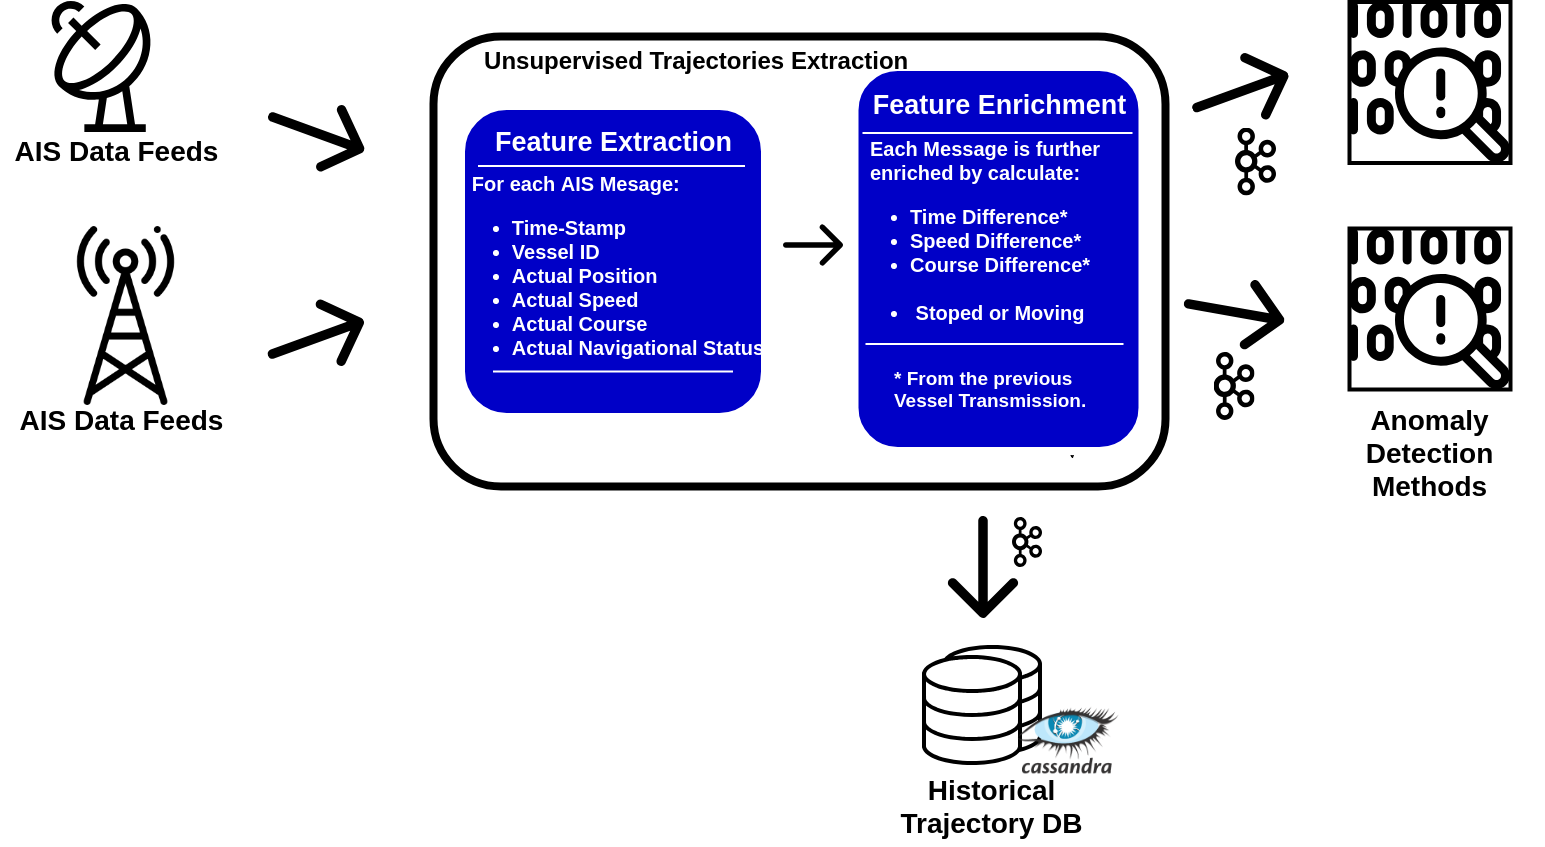
\includegraphics[scale = .25]{figures/UTE.png}
    \caption{Proposed Beta Framework[TODO NEEDS MORE DETAIL THIS IMAGE].}
    \label{fig: Framework}
\end{figure}

In the following subsections, we discuss each module: Data Fusion, Vessel T Extraction, Anomaly Detection and Reporting...

\section{Data}
This section we provide a description, of the different types of Data used and respective sources used. AIS data type was the main source of data for this work, AIS is not-only the most available type data (being the standard for the Maritime positional data), but it was also the data type made available inside the MARISA project.

AIS Historical data can be found in open-access repositories, although AIS Data providers cap the frequency of the messages transitions. This drastically reduces the number of transmitted messages, but also reduces the overall detail of the Data, as lower transmissions rates produce a less certainty of the movement presented by each Vessel. For most general use cases of AIS (e.g. managing a fleet, estimations of time of arrival ...), transmissions rates of 3 Seconds or 30 Seconds, do not provide no information gain, as Vessel kinematics tend to not have abrupt changes, in short periods of time. 

Although, via the MARISA project, we received AIS data via live feeds from Antennas all around the European coast. This Antennas receive the Vessels transmissions broadcast via AIS, till normally a range of 20 Nautical Miles of the shore. The MARISA Live Feeds permit a live test scenario for the proposed Framework, as the live data ingestion of these feeds will represent real case scenarios where the Framework will be Tested.

\subsubsection{Live Data Feeds}
National Marine Electronics Association (NMEA) is a standard communication protocol used by Maritime Sensors such as Accelerometer, Giroscope, GPS receivers, etc.
NMEA being the standard it is the protocol that encapsulates the AIS information, broadcasted by AIS-equipped Vessels. 

TODO SAME AS IN TOP ITS BS

Via the project, we had access to multiple live NMEA feeds, as a way to not only validate our developed methods with live feeds of Nautical data, but also to produce methods that were capable of handling the scale of data that is produced by National feeds.


TODO this might go to chap4

AIS-Receiving stations receive the broadcast AIS information from numerous AIS-equipped Vessels simultaneously. Normally, AIS-Receiving stations are antennas located along the coast line in high grounds, the reception range of these antennas vary, mainly depending on distance to shore, the elevation in which the antenna is located, and the antenna type itself.

Although, the distance in which Stations are capable of receiving AIS messages presents a problem to the Data, as reception ranges vary from 15 Nautical Miles to 50 Nautical Miles, this creates the problem of 

\begin{enumerate}
\item Duplication of Reception:  With the variation of reception ranges, it frequently occurs that multiple stations, receive the same  

TODO - THIS BRINGS TO THE PROBLEM OF MULTIPLE ANTHENAS RECEIVING THE SAME FEED


\item [TODO] disse que havia dois problemas
\end{enumerate}


\section{TODO TOPICS}
DADOS

PRE PROSS

FEATURE EXTRACTION

ARMAZENAMENTO -> CASSANDRA

ANOMALIAS TODA A DEFINICAO 
- FAZER AS QUE TENHO JA...


\section{Unsupervised Vessel Route Extraction}
Representing a Vessel trajectory data, can become a difficulty in the Maritime domain. There are a vast number of solutions described in the literature, which present different solutions for different types of problems. 

A scalable method to represent a trajectory in the Maritime domain, is to look to the trajectory as a whole, this is, as Vessel are obliged to broadcast their AIS information in a semi-continuous rates; knowing that each AIS broadcast message represent the instantaneous kinematic information from a single vessel, aggregating this information over time will represent a vessel trajectory. 

Thus, by identifying each vessel by its MMSI, a trajectory can be considered as the set of AIS messages, identified by the MMSI of each vessel. As each AIS message is time-stamped(contains the time in which was broadcast), our representation of trajectory can be defined as Multivariate Time-Series, this is for each trajectory we have $N$ time-series, in which $N$ represents the number of features considered for each trajectory, further explained in the subsection bellow.

\subsection{Feature Extraction}
AIS data, described in TODO chapter X TODO, presents different possibilities  analysis, as it contains detailed information the actual Vessel Behaviour. Although for this work we focused, on the information that more characterize the Vessel kinematics behaviour, thus decreasing the number of features we have in our Data-Model.



The choice of this features was done with the help of Maritime Knowledge Expert, ... TODO TODO ...

\section{Anomaly Definition}
Nowadays, Vessel abnormal Behaviour is solely analysed by Human Maritime Experts, this is, every Maritime Security Agency assures the coastal surveillance of their territory, by assessing possible threats, and identifying abnormal behaviour. The abnormal Vessel behaviour is then further investigated by Maritime Authorities, which can lead to fines or even criminal charges against the Vessel crew. 

The problem of this current methodology for Anomaly Detection, is that is extremely inefficient. Human analysis only allows a limited number of Vessels that can be analyzed. This problem is aggravated as the number of Vessel at seas is increasing every year in a exponential rate. 

Although as described in Chapter X TODO, Vessel Anomalous Behavior can be quite difficult to formalize empirically. As any possible Anomaly can be caused by a undetermined number of causes, creating a uncertainty that only Maritime Knowledge Experts can assess and determine the truenes of any generated anomaly. Thus, in order to surpass the problem of the definition  an Anomaly, Expert Knowledge from Maritime Experts was accesed under the MARISA project. which firstly was identified what actions would be considered Anomalous 



\chapter{Initial Data-Set Creation} %This was made for FCD subject, 2306 -> this is old... 

%\todo[inline]{annotations +  table different sources of data bases}
The initial AIS database was created from a open-source AIS provided by U.S. coastal waters, ~\cite{MarineCadastre}. The raw database file dbf was downloaded, and transformed to a csv, with the use of a open-source GIS software (QGIS). 
 
Before the download of the data-set it was important to select one area of more interest, as dbf to csv transformations are time consuming, and the a decent sized data-set, was achieved with just one area.

\begin{figure}[H]
	\centering
	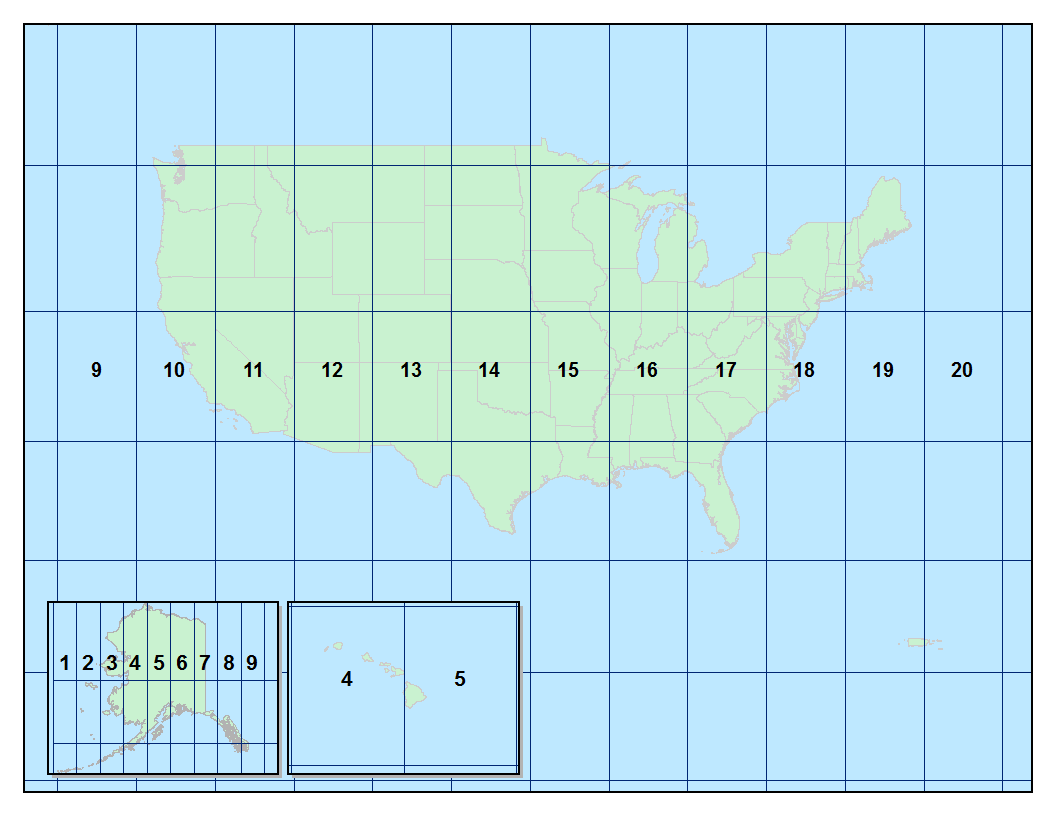
\includegraphics[scale = .35]{figures/UTMZoneMap2014.png}
    \caption{Index map of UTM zones}
    \label{fig: UMT zones}
\end{figure}

The initial selected zone, was zone 10. This zone represents the west coast of the United States, as it is shown in Figure ~\ref{fig: UMT zones}.
The chosen area, represents data whose longitude is from -120 to -126 and latitude is from 30 to 50, from a considerable amount of ships.

%http://www.marinecadastre.gov/ais/

\section{AIS Data}
\label{section: AIS Data}
 With the recent introduction of AIS in the Maritime domain the volume of vessel positional data as exponentially increased, a detailed description of this data, is found in section ~\ref{subsection: chp2_AIS}.

\begin{table}[H]
  \centering
{\small
\begin{tabular}{lrrrrrl}
\toprule
{} &       MMSI &           X &          Y &   SOG &        COG &                Time \\
\midrule
0 &  636081210 & -125.993218 &  48.355773 &  14.3 &  73.300003 & 2014-02-27 13:33:02 \\
1 &  636081210 & -125.985303 &  48.357340 &  14.5 &  73.800003 & 2014-02-27 13:34:23 \\
2 &  636081210 & -125.979437 &  48.358500 &  14.6 &  73.099998 & 2014-02-27 13:35:23 \\
3 &  636081210 & -125.973353 &  48.359692 &  14.7 &  73.000000 & 2014-02-27 13:36:25 \\
4 &  636081210 & -125.965440 &  48.361318 &  15.0 &  73.000000 & 2014-02-27 13:37:46 \\
5 &  636081210 & -125.956733 &  48.363067 &  15.3 &  73.900002 & 2014-02-27 13:39:11 \\
6 &  636081210 & -125.950430 &  48.364153 &  15.7 &  76.099998 & 2014-02-27 13:40:11 \\
7 &  636081210 & -125.944108 &  48.365310 &  15.7 &  74.000000 & 2014-02-27 13:41:10 \\
8 &  636081210 & -125.937763 &  48.366510 &  15.9 &  73.900002 & 2014-02-27 13:42:12 \\
9 &  636081210 & -125.931385 &  48.367660 &  15.9 &  75.000000 & 2014-02-27 13:43:11 \\
\bottomrule
\end{tabular} }
\caption{Example of AIS data transmitted by Vessel, MMSI: 636081210}
\label{Table: TableAIS1}
\end{table}


\section{Route Representation}
Representing the data of a Vessel trajectory, can become a difficulty in the Maritime domain. There are a vast number of techniques described in the literature.

A effective way to represent a trajectory in the Maritime domain, is to look to the trajectory as a whole, this is, as vessel are obliged to broadcast their AIS information in a semi-continuous rates; knowing that each AIS broadcast message represent the instantaneous kinematic information from a single vessel, aggregating this information over time will represent a vessel trajectory. Therefore, knowing the MMSI of a vessel, a trajectory can be considered as the set of AIS messages broadcast, by that vessel, identified by the MMSI.


Thus, a possible definition for a vessel trajectory is a, set of multidimensional-points represented as:
\[TR_{MMSI} = p1, p2, p3, p4, \cdots , pn\]

Where each multidimensional point $p$ is defined as:
\[p = [t, x, y, SoG, CoG]\]


%\todo[inline]{ TODO SE FALTAR DADAS A INTERPOLAÇAO REALIZADA}


%for the Representation of MMSI as a track initially, then the assumption... interpolation of missing SOG and COG values. The use of Haversine formula, justify with as vessel motion is linear and no sudden speed exchanges or route exchanges tend to occur in secounds in the marite traffic, so this .

\section{MARISA Requirements}
\subsection{AIS Signal Loss}
Ships equipped with AIS are obliged to keep the AIS autonomously transmitting AIS messages. A way that ships illegally hide their position and possible what the ships is doing objectively, is by switching off the AIS, or finding ways to block the communications of the AIS transmitter with the coastal receivers.

This creates a problem in the maritime domain, has maritime authorities are constantly finding new ways to discover this illegal activities. A method that looks into historical or new streams of data, was developed. 

This method efficiently uses Data Wrangling techniques, in witch with the aid of powerful Python libraries such as Pandas and Data-Frames, the vessels that don't transmit any information for a parametrized time period, are detected and can be reported for maritime authorities for future investigation.

In table ~\ref{Table: AIS signal loss}, results from the above described method are presented, for this work were conducted on a sub-set of the main data-set, that is, from 50 vessel trajectories, which represents 50,000 AIS messages.

\begin{table}[H]
\centering
\caption{Example of the results, obtained for AIS signal loss, with 50 Ships subset.}
\label{Table: AIS signal loss}
\begin{tabular}{@{}lllll@{}}
\toprule
MMSI & X & Y & Time & Signal Loss Time \\ \midrule
316007330 & -125.990797 & 48.867373 & 2014-02-23 21:43:21 & 18 days 13:53:16 \\
316199201 & -123.375432 & 48.430820 & 2014-02-13 12:26:36 & 11 days 08:18:25 \\
338670018 & -121.378175 & 37.977128 & 2014-02-08 20:18:29 & 7 days 20:06:22 \\
367556504 & -122.495912 & 37.869303 & 2014-02-10 20:45:48 & 7 days 01:57:47 \\
... & ... & ... & ... & ... \\
311240050 & -121.781132 & 30.241660 & 2014-02-06 03:15:42 & 0 days 00:18:39 \\
311240012 & -121.725685 & 30.196453 & 2014-02-08 07:34:12 & 0 days 00:08:30 \\ \bottomrule
\end{tabular}
\end{table}

\subsection{Vessel Rendezvous}
A requirement imposed by the MARISA project, was the development of services, able to detect and generate alarms when two or more vessels are approaching close to each other. This in the maritime world can be called as rendezvous.

The concept of rendezvous in the Maritime world is quite complex, as there are numerous legislation. For the purpose of this work, and because the emphasis is on the alarm generation of possible rendezvous, a simplification of this definition is assumed, therefore: 

~\textbf{Vessel Rendezvous}, for this work is considered as the interception or closeness of two or more vessels, in a configurable time period.

An algorithm was developed in which the a distance ~\textbf{d}, is given as a parameter. For every single Vessel Track, the track is partitioned into time-groups(e.g. a time-group of 5min), ~\textbf{t}, defined also as a parameter. If two or more Vessels, are in the same ~\textbf{t} with a distance smaller than ~\textbf{d}, an alarm is generated for those two vessels.

Figure~\ref{fig: VesselRendevouz2d}, shows two different Vessel Routes, with the axis representing the X and Y coordinate, respectively.

\begin{figure}[H]
	\centering
	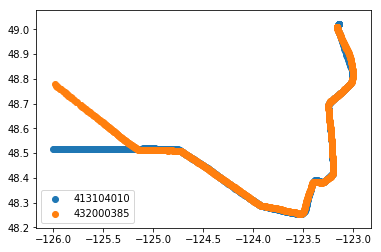
\includegraphics[scale = .8]{figures/VesselRendevouz2d}
    \caption{Two vessel routes}
    \label{fig: VesselRendevouz2d}
\end{figure}

While is obvious that the routes are similar in a positional way, they occur at different times, as is can be see in the figure ~\ref{fig: VesselRendevouz3d} .

\begin{figure}[H]
	\centering
	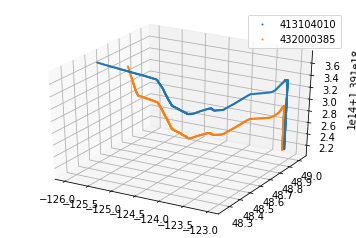
\includegraphics[scale = .9]{figures/VesselRendevouz3d}
    \caption{Two vessel routes, time on Z-axis}
    \label{fig: VesselRendevouz3d}
\end{figure}


   



